\section{Methods of Detector Characterization}

The Detector Characterization (DetChar) group works at the interface 
between the instrument science and data analysis groups. The goal of 
the group is to understand the effects of instrumental noise sources on 
the output of astrophysical searches and mitigate them if possible.

The first step in a detector characterization study is identifying 
noisy or problematic data. These studies can be initiated in a number of ways. 
The three most common are the appearance of 
loud background events in an astrophysical search pipeline, a message from 
the commissioning team regarding instrument performance, or excess noise 
flagged by data quality monitoring software. Section \ref{sec:tools} discusses 
the data quality monitoring software further.

There are a large number of recorded signals used to monitor and control the
interferometers that are not used in astrophysical searches. These auxiliary
channels are considered safe to use for noise characterization because they are
not sensitive to gravitational wave signals. Analyses of auxiliary channels
allow for the identification of systematic noise sources \cite{Smith:2011,Isogai:2010},
such as environmental
disturbances \cite{Effler:2014zpa} or excess motion of auxiliary optics in the
interferometer \cite{GW150914-DETECTORS,InstrumentNoisePaper}. 

Once data with excess noise have been identified, they must be characterized 
in order to track down the source of the noise. A number of questions can 
be asked to characterize the noise. Is the noise transient or a slow 
drift? What is the typical frequency and bandwidth of the noise? Does the 
noise follow a power law in frequency? Does the 
noise have a characteristic shape in the time-frequency plane? Are the 
noisy frequecies of the signal coherent with other signals in the instrument 
such as environmental monitors and optical control signals? 
Is the noise source localized to a specific chamber or does it exist at 
multiple physical locations in the interferometer? Does the characteristic 
frequency match any of the known mechanical resonances in the interferometer? 
If the noise is a slow drift, does it correlate with the slow drift of 
other signals in the interferometer? Does the noise seem highly digital 
or discretized? After gathering all available information about the 
character of the noise and its coupling mechanisms, efforts shift 
toward attempting to mitigate the effects of the noise on search 
pipelines. 

There are two primary ways to mitigate the effects of instrumental noise on 
the output of a search pipeline. The first option, which is highly preferred, 
is to track down the source of the noise in the interferometer and fix the 
problem at its origin. If investigations provided enough information that 
a problem can be traced back to a specific piece of electronics or a 
specific control loop, the problem can be fixed at the source. However, 
this is not always possible since instrument noise can be difficult to 
pin down and hardware repairs are often too invasive to perform during 
an observing run.

If the problem cannot be fixed at the source, the second option is to 
remove the problematic data from the astrophysical analyses. 
When a significant noise source has
been identified using auxiliary channels and cannot be repaired immediately, 
a data quality flag can be generated
to indicate times when the output data from the interferometer is not nominal
\cite{Nuttall:2015dqa,S6DetChar,GW150914-DETCHAR,Amaldi}.
Data quality vetoes are discussed further in section (??).  
If possible, it is always preferable to fix a problem at the source. 

\section{Tools and algorithms}\label{sec:tools}

Identifying and characterizing instrument noise is facilitated by a 
suite of software tools and algorithms designed to flag data with 
excess noise and help correlate this noise with other signals in the 
interferometer. The major tools required for understanding the data 
quality investigations in this thesis are discussed below. 

\subsection{Omicron}

One way to quantify the amount of excess noise in $h(t)$ is to look 
for times where the signal contains excess power using 
Omicron, a burst algorithm. 
The first stage of the Omicron pipeline applies a set of signal conditioning 
processes, including a whitening filter, a high pass filter, and a downsampling 
process to $h(t)$. Once the data have been whitened they are projected into 
a sine-Gaussian basis. Each sine-Gaussian basis function is defined 
by a central time, $t_0$, a central frequency, $f_0$, and a Q-factor, 
which is defined as \cite{McIverThesis}  
\begin{equation}
Q = \frac{f_0}{\Delta f} = 4\pi f_0 \Delta t,
\end{equation} 
where $\Delta t$ is the time duration of the sine-Gaussian and 
$\Delta f$ is the bandwidth of the sine-Gaussian. Using these parameters, 
each sine-Gaussian basis function can be represented as a tile in the 
time-frequency plane centered around $t_0$ and $f_0$, where the width of 
the tile is determined by the time duration 
and height of the tile is determined by the frequency bandwidth. 

For each 
of these tiles, the energy is measured and compared to the median tile 
energy. If there is an excess of energy in a given tile relative to the 
median tile energy, a signal-to-noise ratio (SNR) is calculated and a trigger 
is generated to annotate the event. For each trigger, the SNR, central time, 
central frequency, duration, bandwidth, and Q of the tile are recorded. 

Once the data have been decomposed into the full set of basis functions, the 
resulting set of triggers is sent through a clustering algorithm. This is 
necessary because the set of sine-Gaussians is an overcomplete, 
non-orthogonal basis and a single event in the data can generate multiple 
triggers corresponding to different values of $t_0$, $f_0$, and Q. The 
resulting clustered triggers define the peak time, peak frequency, and 
SNR of a cluster as the central time, central frequency, and SNR of the 
most significant tile in the cluster. 

The most useful way to visualize the output of Omicron is in the 
time-frequency-SNR plane, sometimes referred to as a 'glitchgram', 
where each trigger is represented as a point 
in a scatterplot. Figure \ref{fig:glitchgram} shows an example set of 
Omicron triggers in the time-frequency-SNR plane. Each dot represents 
a trigger at a certain peak time and peak frequency. The color of each 
dot represents the SNR of that trigger. 

In Gaussian noise, the SNR of a 
given trigger is not expected to exceed 8. In this example, there are a number 
of triggers with SNR $> 8$, some with noticeable structure and some that seem 
more randomly scattered, that represent noise in the output of the interferometer. 
For example, there are numerous triggers between 10-20 Hz that represent excess noise at 
these frequencies, likely due to scattered light in the 
interferometer. There is a line of triggers at just above 2kHz that indicates 
a noise source with a constant peak frequency whose amplitude is being modulated 
and a high SNR is being reported. There is also a scattering of points with high 
SNR that are not as structured as the previous two examples, each one likely due 
to an individual loud glitch rather than a constant, systematic noise source.

\begin{figure}[ht!]
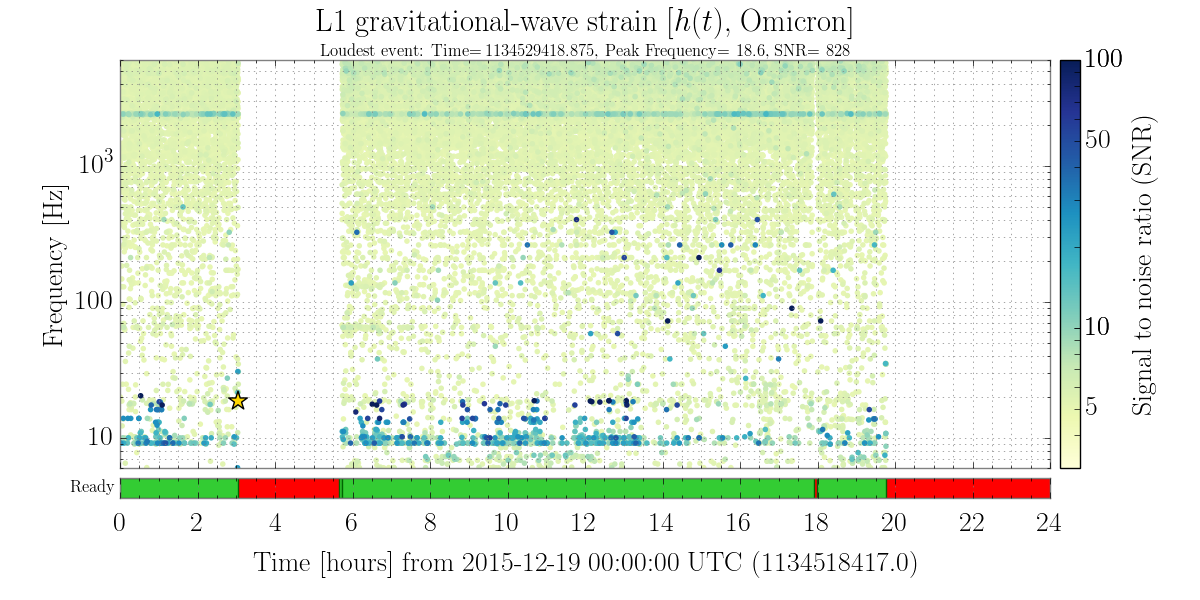
\includegraphics[width=\textwidth]{figures/detchar/Omicron-Dec19}
\caption[Omicron time-frequency-SNR plot]{Time-frequency-SNR plot of Omicron triggers, %
         often referred to as a 'glitchgram'. Each dot on this plot represents an %
         event in $h(t)$ that was recorded with a peak time, peak frequency, and SNR. %. 
         In Gaussian noise, all triggers on %
         this plot would have an SNR $< 8$. Since this plot is generated using real %
         detector data from O1, there are structures of loud triggers that indicate %
         populations of noise transients. For example, the clusters of triggers %
         between 10-20 Hz that likely represent scattered light in the interferometer. %
         }
\label{fig:glitchgram}
\end{figure}

The results of Omicron are a commonly used and extremely valuable tool 
for characterizing the noise in the instrument. A cursory glance at 
Figure \ref{fig:glitchgram} identifies 3 populations of noise in 
the instrument, each of which can be followed up on individually 
to discover both the source of the noise and its effect on astrophysical 
searches. Omicron triggers can also be used in statistical analyses to 
find correlated noise between auxilary channels and $h(t)$. An often used 
example of this, Hierarchichal Veto, is discussed below. 

\subsection{Hierarchichal Veto}

One tool that we have often used in Detector Characterization to look 
for time coincidence between noise transients, or 'glitches', in auxilary 
channels and the output of the interferometer is Hierarchical Veto (Hveto) 
\cite{Smith:2011}. 
Typically, Hveto is used to compare a channel that potentially contains 
gravitational wave signals, denoted $h(t)$, and an auxiliary channel 
that does not have direct astrophysical implications. Hveto counts 
the number of coincident triggers between two time series using a 
user-defined time window centered around each trigger in the auxiliary 
channel. 
Figure \ref{fig:hveto-aux} shows an illustration of auxiliary channels 
with noise transients that are coincident with noise in $h(t)$. Hveto 
iterates over all auxiliary channels to search for noise that is coincident 
with noise in $h(t)$ in a statistically significant way.

\begin{figure}[ht!]
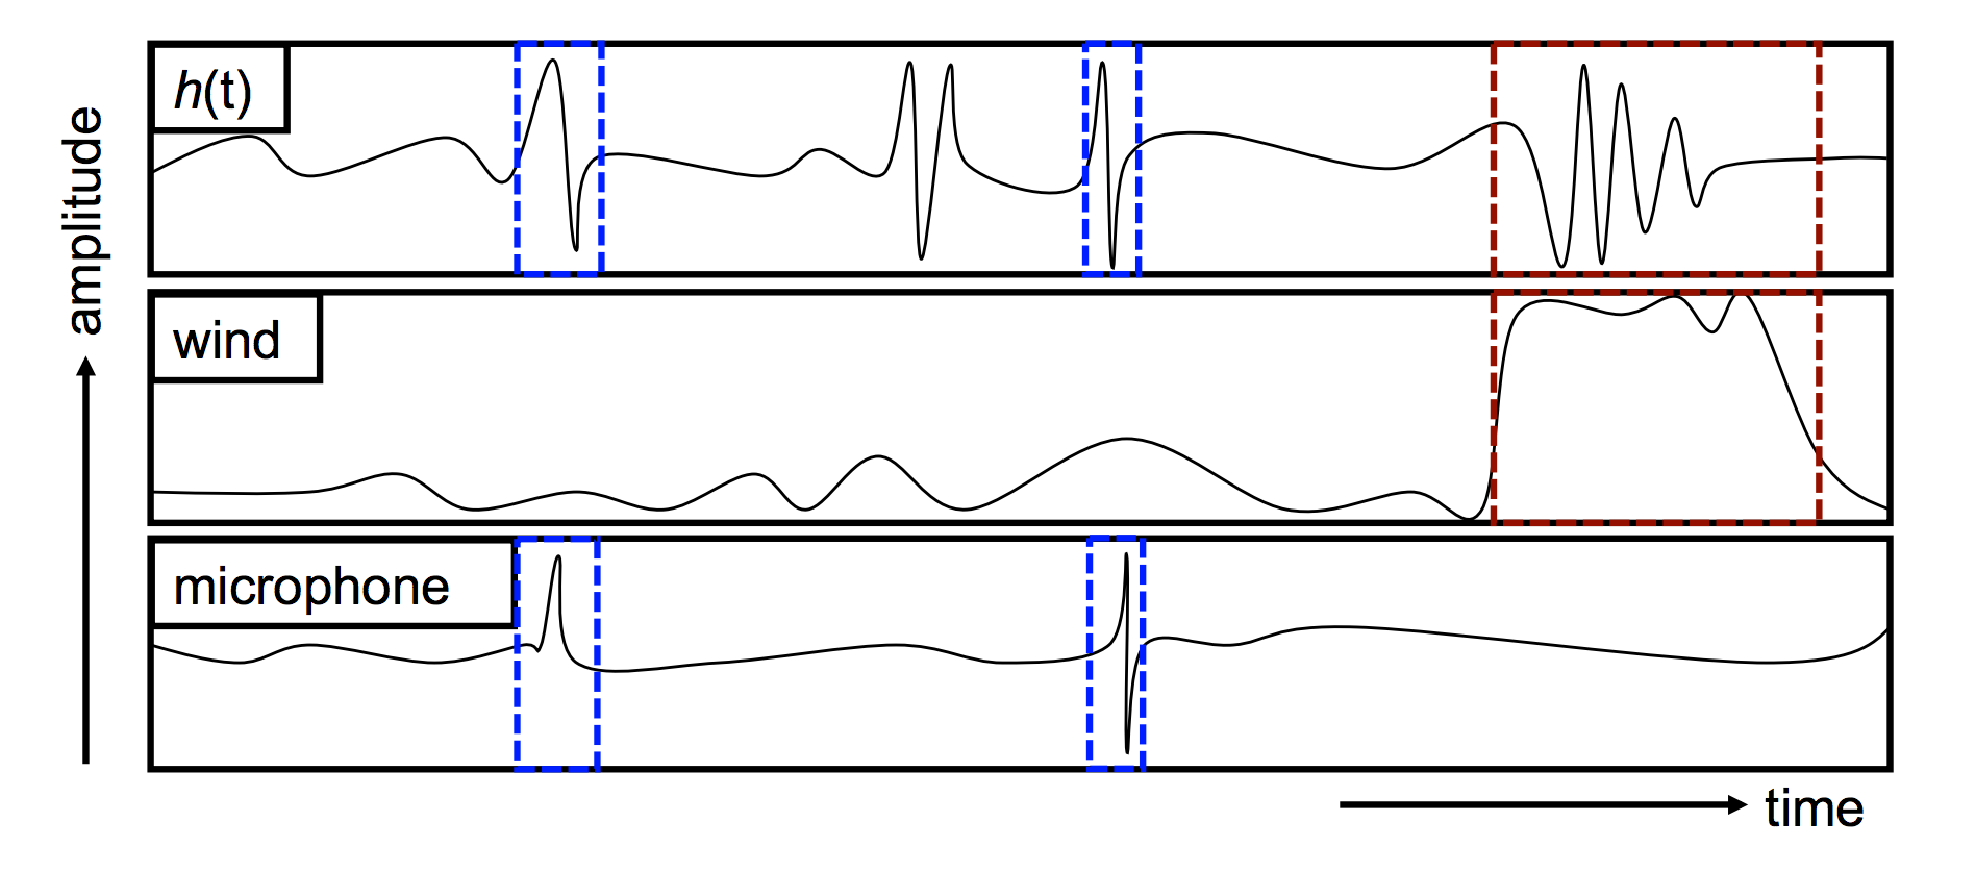
\includegraphics[width=\textwidth]{figures/detchar/hveto_example}
\caption[Example of coincident noise]{A time-series illustrating coincident noise %
         between auxiliary channels and $h(t)$. The top panel is $h(t)$, which contains %
         multiple noise artifacts of varying duration. The middle panel is a readout of %
         wind speed on site, which shows an elevated period coincident with a longer duration %
         burst of noise in $h(t)$. The third panel is a readout of a microphone on site, %
         which shows two glitches that are coincident with bursts in $h(t)$. If noise in %
         these auxiliary channels are coincident with noise in $h(t)$ in a statistically %
         significant way, the noisy data in $h(t)$ can be removed. Figure reproduced from %
         \cite{Smith:2011}.
         }
\label{fig:hveto-aux}
\end{figure}

The figure of merit returned by Hveto for each auxiliary channel 
after comparison to $h(t)$ is called significance.
Significance answers the following question: how unlikely is it that 
the coincident triggers in these two channels were the result of 
two arbitrary Poisson processes occurring in each channel? 
More specifically, given two arbitrary Poisson processes, how 
unlikely is it that we measure $n$ or more coincident triggers 
given that expected number of coincidences from random chance is $\mu$?

Significance is calculated as \cite{Smith:2011},
\begin{equation}
S = -\log_{10} (\sum\limits_{k = n}^{\infty} P(\mu,k)),
\end{equation}
where $n$ is the number of coincidences found between the two channels 
during the total analysis time and $P(\mu,k)$ is the Poisson probability 
distribution function,
\begin{equation}
P(\mu,k) = \frac{\mu^{k}e^{-\mu}}{k!},
\end{equation}
where $\mu$ is the expected number of coincidences between triggers in 
$h(t)$ and the auxiliary channel based solely on chance, which is estimated as,
\begin{equation}
\mu = \frac{N_{h}N_{aux}T_{win}}{T_{tot}},
\end{equation}
where $N_{h}$ and $N_{aux}$ are the number of triggers in $h(t)$ and a 
given auxiliary channel respectively, 
$T_{tot}$ is the total analysis time, and $T_{win}$ is the length of the 
coincidence window used.

A high value of significance indicates that the triggers in the channels 
were very often coincident in time and that there is a very small probability 
that their intersection is a product of random chance. This is a very useful 
measure when we are searching for auxiliary channels that might have some 
noise coupling into our output channel. A significance value of up to 5 is 
often observed in channels with no causal relationship to $h(t)$ \cite{Smith:2011}, 
which is a useful threshold for identifying effective vetoes.

Another interesting figure of merit used for a given comparison Hveto is 
the ratio of $\frac{efficiency}{deadtime}$. Efficiency is defined as the 
percent of triggers vetoed from $h(t)$ during a round of vetoes. Deadtime 
is defined as the percent of total analysis time removed from $h(t)$ during 
a round of vetoes. A ratio of 1 is what we would expect from vetoing time 
at random, indicating no strong time correlation between triggers in the 
two channels. A high value of this ratio, which is ideal, indicates that 
we are vetoing a large number of triggers while maintaining a high percentage 
of our analysis time. This means that the triggers are often close enough 
in time that we can catch a large number of triggers using a small time window.

The deeper utility of Hveto is made evident when a channel is found to have 
a strong correlation with $h(t)$. 
When Hveto discovers an auxiliary channel that has a strong correlation 
with $h(t)$, which is called the round winner, it removes all of the time 
windows surrounding 
auxiliary channel glitches and recalculates the significance of the list of 
auxiliary channels. If a channel's significance has dropped after this removal 
of time, it must have had a large amount of glitches coincident with the 
round winner. The change in significance of each channel is displayed on a 
figure called a `drop-plot`. This is one of the most powerful features of Hveto
 - the ability to find families of channels that often glitch at the same time. 

Ideally, the list of significant channels displayed on the drop-plot will be 
able to localize the issue to a specific subsystem or area of the IFO. 
For example, if a channel representing the alignment of the input mode 
cleaner has glitches that are strongly correlated to $h(t)$, it would be 
interesting to look at the drop-plot and find out what other channels are 
glitching at the same time (suspensions, laser power, etc.).
From there, the issue can be investigated and brought to the attention of 
commissioners for repair or physical inspection. This is not always possible 
as sometimes the cause of the glitches is unclear, but identifying times of 
poor data quality is still useful.

Using Hveto, we can monitor auxiliary channels to find and remove glitches 
in $h(t)$ that would otherwise pollute a gravitational-wave analysis. Removing 
these glitches serves multiple purposes for the search pipelines. Removing 
high SNR glitches cleans up search backgrounds and allows the search 
pipelines to claim a lower SNR threshold for potential detections. A lower 
SNR threshold implies a larger volume for astrophysical analysis. Removing 
glitches reduces the potential for false alarms in the search pipelines, 
which in turn increases the confidence of eventual detections.

\section{Instrumental Detector Characterization Studies}

\subsection{Analog-to-Digital Conversion}

Advanced LIGO interferometers are controlled in real-time using a digital 
control system installed on a series of computers referred to as front end 
computers.  This system overall is referred to as the Front End Control 
(FEC) subsection of the more expansive Control and Data System (CDS).  
In a control loop, the FE computers must be capable of reading in an 
analog signal from the interferometer (position measurements, error signals, 
coil currents, etc), digitally sampling that analog signal, using these now 
digital values in a series of control algorithms, and outputting an analog 
control signal to send back into the interferometer.

The process of digital sampling is handled by an analog-to-digital 
converter (ADC) and the process of analog output is handled by a 
digital-to-analog converter (DAC).  Since these converters are linearly 
mapping a continuous signal onto a discrete range, they are limited by 
their digital bit depth.  For example, a 16 bit ADC is only capable of 
representing $2^{16}$ discrete values, or a range from zero to 65536.  
This range is often centered around zero, giving the ADC the capability 
to handle a range of $\pm32768$.  An incoming analog signal is mapped 
onto this range and converted into a digital signal.

For example, in sampling an analog signal with a range of $\pm20V$, 
10V would be mapped to 32768 digital counts and -10V would be mapped 
to -32768 digital counts with all 
of the intermediate voltage values being linearly mapped to the range. This 
means our digital system would recognize a discrete step size of 
10V/32768 counts $\approx 305 \mu $V/count.

Looking at the system described above, we must be aware of how our system 
is going to react when our analog input signal exceeds the intended maximum 
value of 10V (e.g., an 11V input). The ADC has already assigned its maximum 
digital value to 10V. This is called a digital overflow. In this case the ADC 
will continuously output its maximum value as it has no way to map 11V into 
a discrete value. The same process can occur in a DAC when a digital signal 
is sent out at the maximum allowed digital value. The resulting analog signal 
will be railed at the maximum output value of the DAC, creating a sharp corner 
in the output signal as it flattens out. 

If the digital system is not able to correctly sample and understand an analog 
error signal, it is easy to imagine a scenario where the reponse of the digital 
system and the output control signal are not able to complete the control loop 
as designed. This may cause glitches or misalignments in the interferometer.
We must also consider the fact that many ADCs are calibrated to reflect the 
intended dynamic range of an optic.  If a saturation is occurring, there is 
a good chance that an optic has moved beyond this intended dynamic range, which 
also may cause glitches or misalignments.

The ADCs and DACs are monitored by a series of auxiliary channels, which are 
automatically generated in the front-end system. These auxiliary channels 
monitor each ADC and DAC channel and note when any of the channels has reached 
its digital limit. These channels can be used to generate flags that mark 
ADC and DAC overflows, which can be compared with glitches in $h(t)$ to 
search for glitch mechanisms driven by overflows. These channels can also 
be used to flag any large glitches that cause digital overflows so that they 
can be removed from astrophysical searches. 

Figure \ref{fig:dac-overflow} shows an example of a large glitch that caused 
a digital overflow and was removed from gravitational wave analyses. Figures 
\ref{subfig:strain-dac-overflow} and \ref{subfig:esd-dac-overflow} show a 
large glitch in $h(t)$ and the response of a drive signal that controls 
the motion of ETMY respectively. The signal in \ref{subfig:esd-dac-overflow}, 
which is supposed to be controlling the motion of ETMY, hits its digital 
limit during this glitch. Figure \ref{subfig:etmy-dac-overflow} shows the 
auxiliary channel that monitors this digital overflow incrementing as 
it witnesses the digital overflow. 

\begin{figure}[ht!]%
\centering
\subfloat[]{
  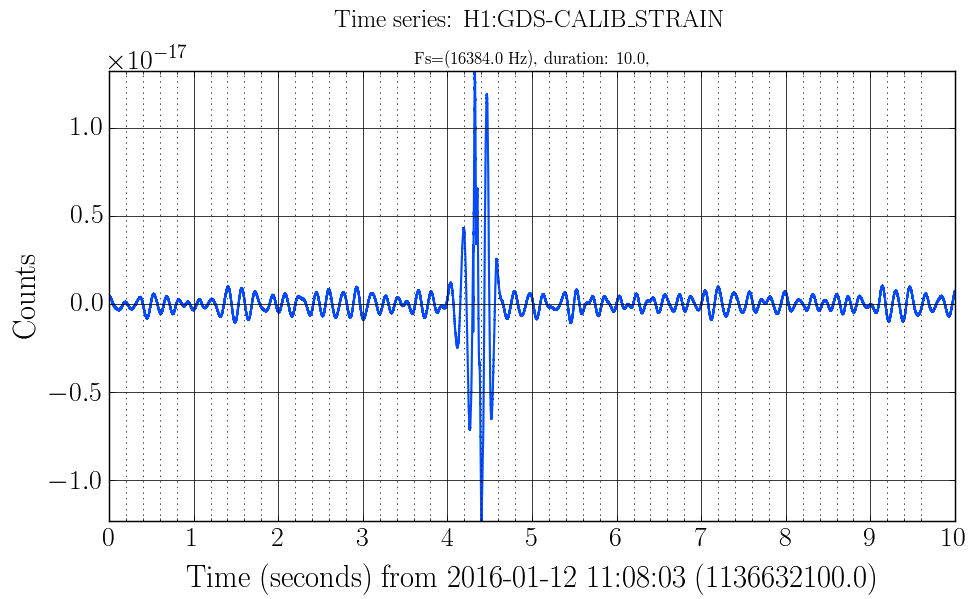
\includegraphics[width=0.495\textwidth]{figures/detchar/strain-dac-overflow}
  \label{subfig:strain-dac-overflow}
  }
\subfloat[]{
  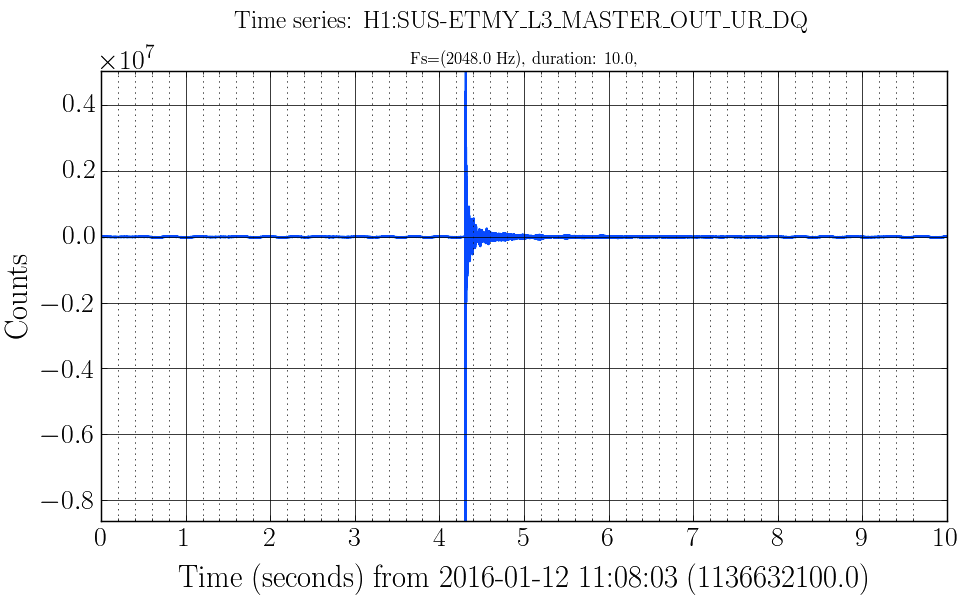
\includegraphics[width=0.495\textwidth]{figures/detchar/esd-dac-overflow}
  \label{subfig:esd-dac-overflow}
  }

\subfloat[]{
  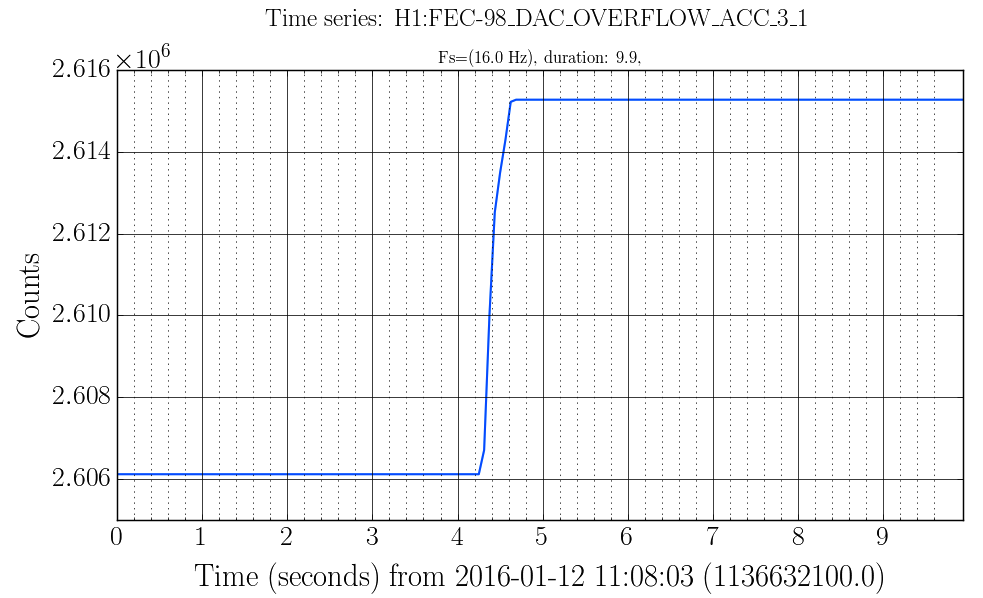
\includegraphics[width=0.495\textwidth]{figures/detchar/etmy-dac-overflow}
  \label{subfig:etmy-dac-overflow}
  }
\caption[ETMY saturation]{Timeseries of an ETMY drive signal saturation in the 
         H1 detector. Figure \ref{subfig:strain-dac-overflow} shows a glitch in 
         the calibrated $h(t)$ channel. Figure \ref{subfig:esd-dac-overflow} shows 
         the response to this glitch in the drive signal used to control the bottom 
         stage of ETMY and actuate on the DARM degree of freedom. This signal hits 
         its digital overflow point at its peak and has no more dynamic range. 
         Figure \ref{subfig:etmy-dac-overflow} shows the front end channel responsible 
         for monitoring digital overflows of this particular ETMY drive signal. 
         Since the witness channel is cumulative, overflows can be identified by 
         flagging any time in which this witness channel is increasing. }
\label{fig:dac-overflow}
\end{figure}

This method was used throughout O1 to generate data quality vetoes that 
were distributed to the Burst and CBC searches. The first veto that was 
generated this way was used to flag DAC overflows of the ETMY drive signal, 
as demonstrated 
in Figure \ref{fig:dac-overflow}. The other veto generated in this framework 
was used to flag ADC overflows in the OMC DC photodiode used as the error 
point of the DARM control loop. 

\subsection{Suspension DAC calibration glitches}

A common glitch mechanism throughout ER6 was due to calibration errors in 
digital-to-analog converters (DACs) responsible for providing analog signals 
to the aLIGO suspensions. The aLIGO suspension subsystem uses 18-bit DACs 
to interact with the optics in the interferometer. These 18-bit DACs are 
created by combining a 16-bit DAC with a 2-bit DAC inside of the same 
electronics box. The 2-bit DAC is responsible for the two highest order 
bits of the output, while the 16-bit DAC is responsible for the 16 lowest 
order bits of the output. If the 16-bit DAC and 2-bit DAC have not had 
their output voltages carefully calibrated, there will be a voltage discontinuity 
at the output of the DAC when engaging the 2 highest order bits. 

Since these DACs use the two's complement 
representation for signed binary numbers, there are two critical points 
where the two highest order bits of the DAC become necessary. The highest 
order bit is used to indicate negative numbers, so an output discontinuity 
is expected when transitioning from a positive number to a negative number, 
that is, crossing through a value of zero.  
The other bit from the 2-bit DAC is used to represent large output values and 
engages when the DAC needs to express a value which is unable to be 
represented by a 16-bit DAC alone. As such, we also 
expect to see discontinuities when the DAC output crosses $\pm2^{16}$. 

The fact that this discontinuity existed in suspension subsystem was 
particularly problematic, as the suspension DACs are used to directly 
actuate on mirror positions and optical cavity lengths. Any time a 
suspension DAC crossed one of these problematic output values, it would 
actuate on the optics with a step function and cause a glitch in the 
optical cavity length. Figure \ref{fig:DAC-glitch} shows an example of 
this issue where the DAC providing actuation signals to the power recycling 
mirror (PRM) is crossing through zero and there are associated glitches 
visible in the length readout of the power recycling cavity.

\begin{figure}[ht!]%
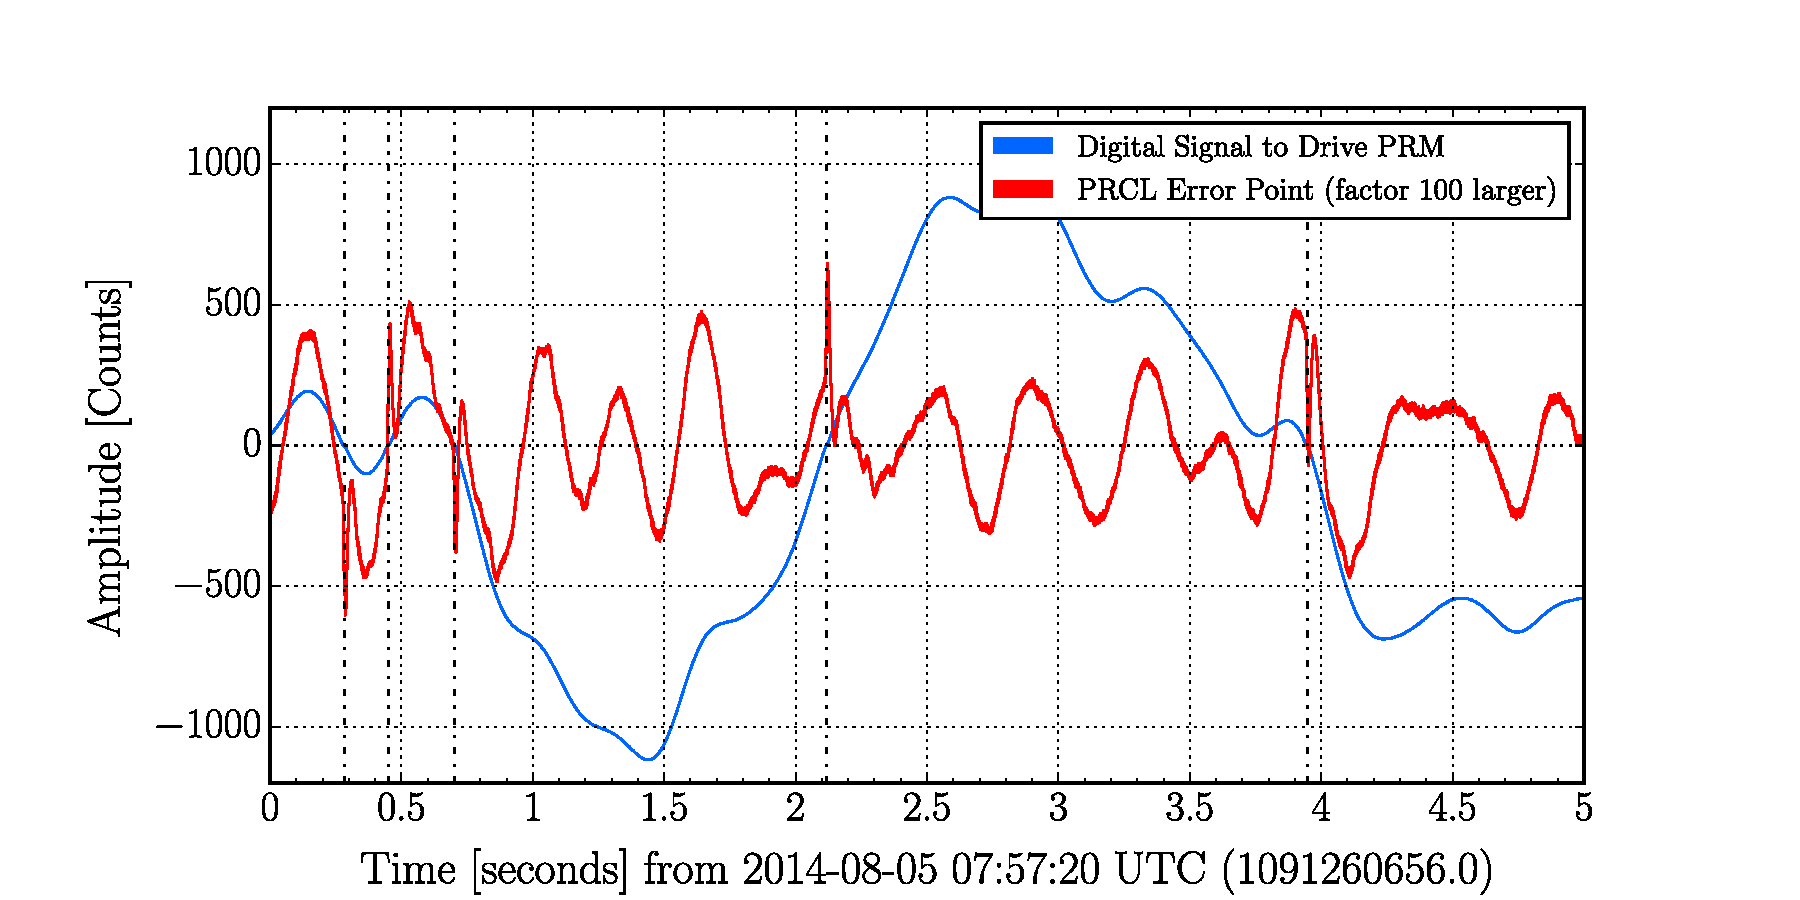
\includegraphics[width=\textwidth]{figures/detchar/PRCL-DAC-glitch}
\caption[DAC glitches in PRCL]{A timeseries plot showing the effects of %
         DAC calibration glitches. The red trace shows the digital drive %
         signal being sent to the digital-to-analog converter. The blue %
         shows the resulting power recycling cavity motion rescaled by a %
         factor of 100. When the drive signal crosses %
         through a value of zero, the output of the DAC experiences a %
         discontinuity, leading to a glitch in the power recycling cavity %
         length.}
\label{fig:DAC-glitch}
\end{figure}

The effects of this issue were visible in the $h(t)$ channel during ER6. 
The most problematic culprit was the DAC that applied actuation directly 
to the optics of the ETMs, effectively pushing directly on the DARM degree 
of freedom and causing glitches in $h(t)$. These calibration errors manifested 
themselves as a population of glitches in $h(t)$ recovered by Omicron in the 
20-100 Hz range. This is a very damaging frequency range for CBC searches, 
which hope to accumulate significant SNR in the region from 30-500 Hz.  
This population of low frequency glitches was obvious in an Omicron 
time-frequency scatter plot and was considered a significant noise source 
throughout the sixth engineering run.

Figure \ref{fig:vetoed-DAC} shows the result of an Hveto run that looked 
for time correlations between Omicron triggers in $h(t)$ and times when 
the ETMY drive signal crossed through a value of $2^{16}$. The blue dots 
represent all Omicron triggers in $h(t)$. The red crosses indicate those 
that were coincident with the ETMY drive signal crossing $2^16$. The 
population of low frequency glitches with SNR $>$ 8 was shown to be 
coincident with the drive signal transitions. This veto 
was very statistically significant, as shown in Table \ref{table:etmy-dac-hveto}. 
The significance 
of 192.5 indicates that the probability of these coincidences being due 
to noise alone is negligible. The effiency:deadtime ratio of 27 indicates 
that these glitches were removed with very small time windows (0.2s) 
and very little instrument uptime was removed in the process.

\begin{figure}[ht!]%
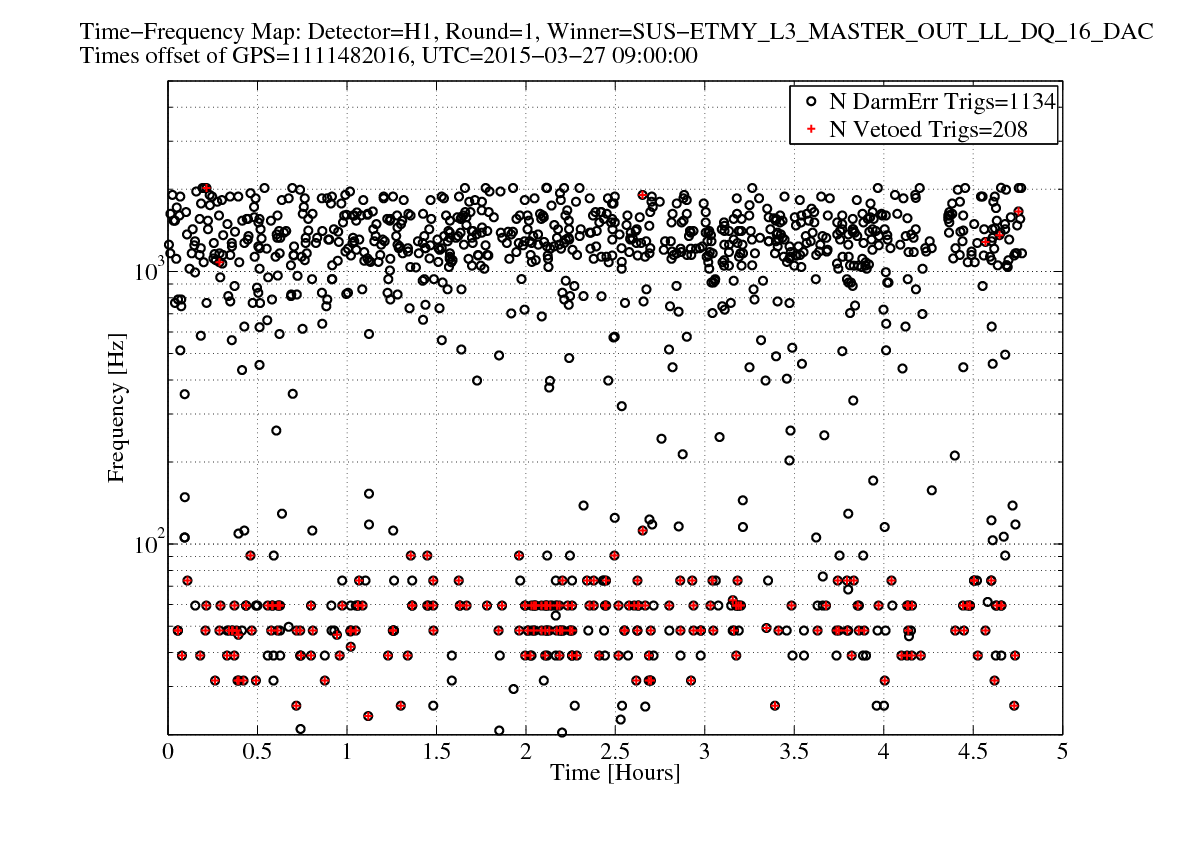
\includegraphics[width=\textwidth]{figures/detchar/vetoed-DAC-glitches}
\caption[Vetoed DARM triggers from DAC calibration]{A time-frequency %
         visualization of Omicron triggers in the H1 $h(t)$ channel. % 
         The black circles indicate glitches in the DARM degree of freedom, %
         each with a central time and central frequency. The red crosses %
         indicate that a given trigger was vetoed by an auxiliary channel %
         trigger which was found to be statistically significant using Hveto. The %
         auxiliary channel triggers in this case indicate that the drive signal %
         on the bottom stage of ETMY has crossed a value of $2^{16}$. The %
         population of glitches between 20 - 100 Hz is highly coincident %
         with these crossings of $2^{16}$, indicating that they are caused %
         by DAC calibration errors on this optic.}
\label{fig:vetoed-DAC}
\end{figure}

\begin{table}[ht!]%
 \footnotesize 
 \begin{center}
  \begin{tabular}{cccccc}
  \hline
  Channel & \begin{tabular}{@{}c@{}} Time \\ window (s) \end{tabular} & 
            \begin{tabular}{@{}c@{}}SNR \\threshold \end{tabular} & 
            Significance & Efficiency \% & Deadtime \% \\ 
  \hline
  \begin{tabular}{@{}c@{}}ETMY drive signal \\ crosses $2^{16}$ \end{tabular} & 
  0.2 & 8 & 192.5 & 18.3 &  0.674 \\
  \hline
  \end{tabular}
  \end{center}
  \caption[HVeto results for ETMY DAC glitches]{Hveto results for ETMY DAC glitches}
  \label{table:etmy-dac-hveto}
\end{table}

To fully understand the scope of this problem, the Detector Characterization 
group developed software that searched through the output of all suspension 
DAC digital output signals and marked times when they crossed 0 or $\pm2^{16}$. 
These marked times were converted into trigger files and sent through Hveto 
to look for correlations between crossings of critical values and glitches 
in DARM as identified by Omicron. Through this method, we were able to identify 
which optics were experiencing DAC calibration glitches that had a coupling 
mechanism into DARM.

There were two approaches taken in an effort to mitigate these DAC glitches. The 
first was to introduce offsets into the suspension drive signals so that they 
did not cross through a value of zero. This did solve the problem temporarily, 
but at the cost of a significant portion of the dynamic range of the output 
actuation. The more permanent fix was to run a calibration routine 
that resolved the issue between the 16-bit and 2-bit DACs. This was 
successful, though it had to be run on a weekly basis during site maintenance 
because the calibration tended to drift away from its nominal point after 
2-3 weeks of operation.

During the first observing run, the systematic check of all suspension DAC 
digital output signals was performed again and the resulting triggers were 
sent through Hveto. This study revealed that the calibration process was 
successful; there was no evidence of residual DAC calibration glitches that 
had any noticeable coupling into $h(t)$. The only signal that had any 
significant correlation with glitches in $h(t)$ was not causally sensible. 
Large glitches $h(t)$ were driving the ETMX actuation signal through a value of 
$2^{16}$, which resulted in crossings of $2^{16}$ that were coincident in time 
with glitches in $h(t)$, but weren't representative of calibration errors.

\textcolor{red}{Discuss Hveto results}

\subsection{RF beatnote whistles}

During Advanced LIGO's commissioning,
a population of glitches appeared in both the L1 and H1 interferometers which 
came to be known as 'whistles' or 'RF whistles'. These glitches were the 
intermodulation products of two RF oscillators; a nonlinear mixing between two 
RF oscillators produced a beatnote signal whose frequency was equal to the 
difference in frequency between the two oscillator signals. Whistle glitches 
occur when two oscillator signals drift and cross each other in frequency. 
If one oscillator 
is drifting in frequency and another oscillator is at a fixed frequency, 
the beatnote generated between them will decrease in frequency as the 
oscillator signals become closer in frequency and then increase in frequency 
as they cross each other and drift away. 
As such, these glitches 
had a characteristic shape, beginning at high frequency and sweeping down 
in frequency through the detection band before turning around and 
sweeping back up to high frequencies. Figure \ref{fig:whistle-spectrograms} 
shows a time-frequency representation of whistle glitches in both the L1 and H1 
interferometers ?? . These show the characteristic 'V' or 'W' shape produced 
when two oscillators drift past one another and have nonlinear mixing.

\begin{figure}[ht!]%
\centering
\subfloat[]{
  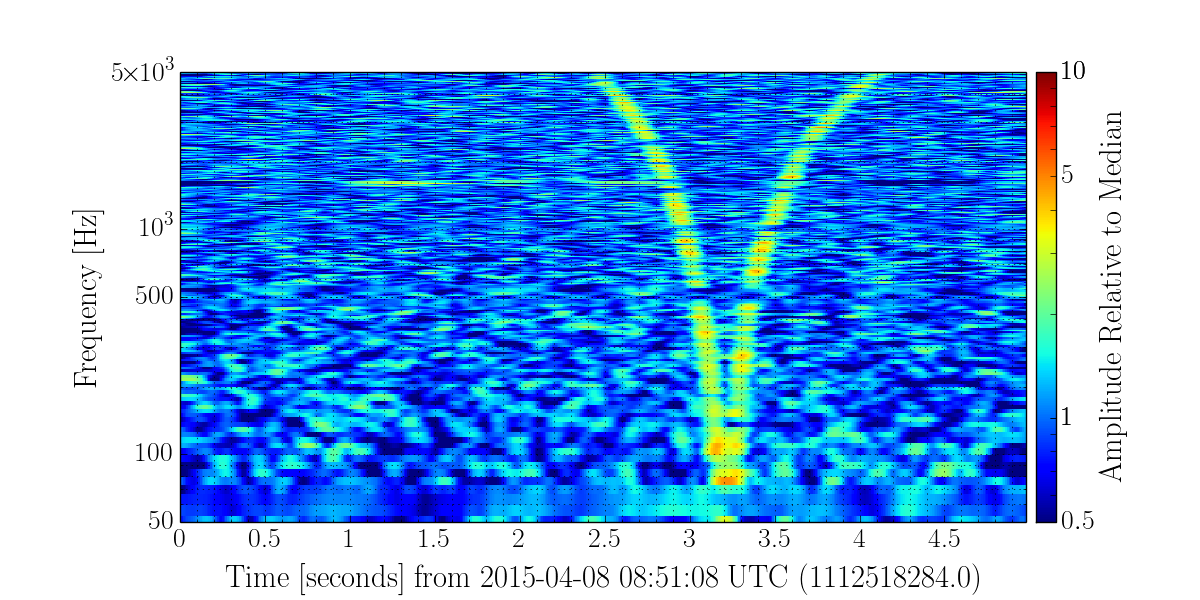
\includegraphics[width=\textwidth]{figures/detchar/Spectrogram_Whistle_LLO}
  \label{subfig:llo-whistle}
  }
  
\subfloat[]{
  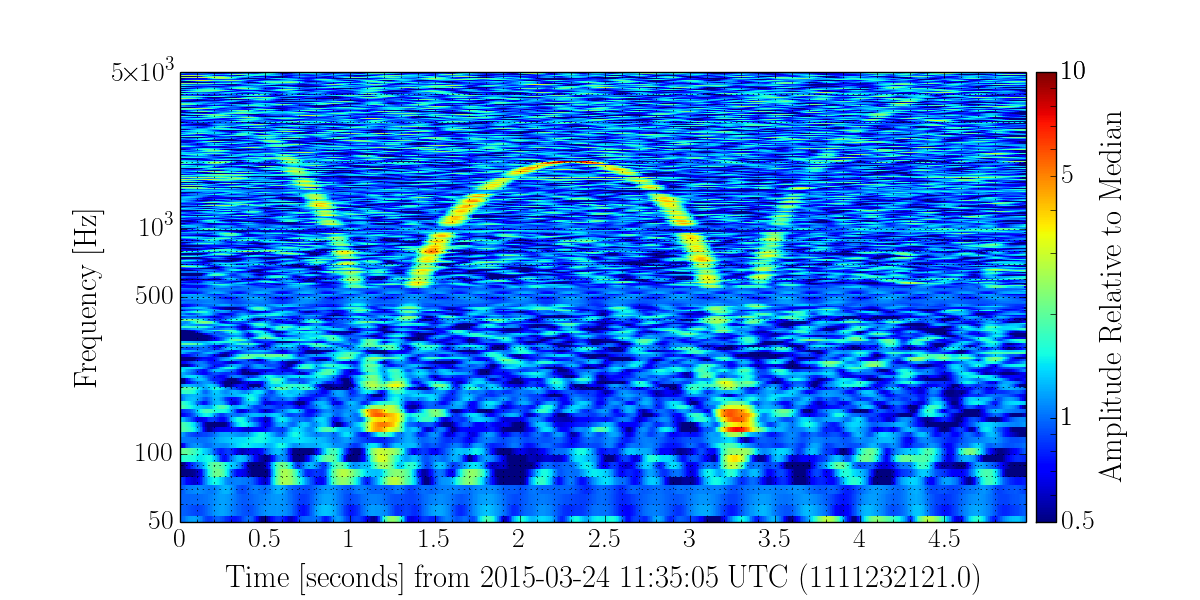
\includegraphics[width=\textwidth]{figures/detchar/Spectrogram_Whistle_LHO}
  \label{subfig:lho-whistle}
  }
\caption[Spectrograms of RF whistles]{Time-frequency spectrograms of RF whistles at %
         both LLO and LHO. Figure \ref{subfig:llo-whistle} shows a %
         whistle at LLO sweeping down from the kHz range and into the detection band %
         where it interferes with searches for gravitational waves. Figure %
         \ref{subfig:lho-whistle} shows a double whistle whistle at LHO where the %
         two oscillators drifted back and forth across one another and caused two %
         glitches in the detection band.}
\label{fig:whistle-spectrograms}
\end{figure}

Voltage controlled oscillators (VCOs) are oscillators whose frequency can 
be tuned using an input voltage. These oscillators are used in control 
loops throughout the aLIGO interferometers. One particular example of this 
is the control loop which locks the frequency of the input laser to the 
length of the input mode cleaner to guarantee a resonant optical cavity and 
effective mode cleaning. A signal representing the changing length 
of the input mode cleaner is read out using the Pound-Drever-Hall (PDH) technique ?? . 
This signal is used as the input to a VCO, which produces a 
signal whose frequency is a proxy for the length of the input mode cleaner. 
This signal is used as the set point in the frequency stabilization loop that 
controls the frequency of the input laser light. Through this path, the length 
of the input mode cleaner is used to set the frequency of the input laser light. 

The signal that represents the length of the input mode cleaner was found to 
be a good witness for RF whistle glitches. Figure \ref{fig:darm-whistle-hist} 
shows the rate of Omicron triggers, which represent generic transient noise in 
$h(t)$, as a function of the length of the input mode cleaner. The length of 
the input mode cleaner is in kHz as it is an error signal used to set the 
frequency detuning of the VCO. The red curve represents the distribution in 
the absence of whistle glitches. There is no value for which noise transients in 
$h(t)$ seem more likely to occur; the rate of glitches seems Gaussian distributed 
as the length of the input mode cleaner fluctuates about the set point of the 
control loop. The blue curve represents the rate of transients 
when RF whistle glitches are occurring. In this case, there are three preferred 
frequencies where it seems that noise transients in $h(t)$ have a tendency to 
occur. This indicates that there is a relationship between specific values of 
the length of the input mode cleaner and the presence of whistle glitches in the 
interferometer. 

\begin{figure}[ht!]%
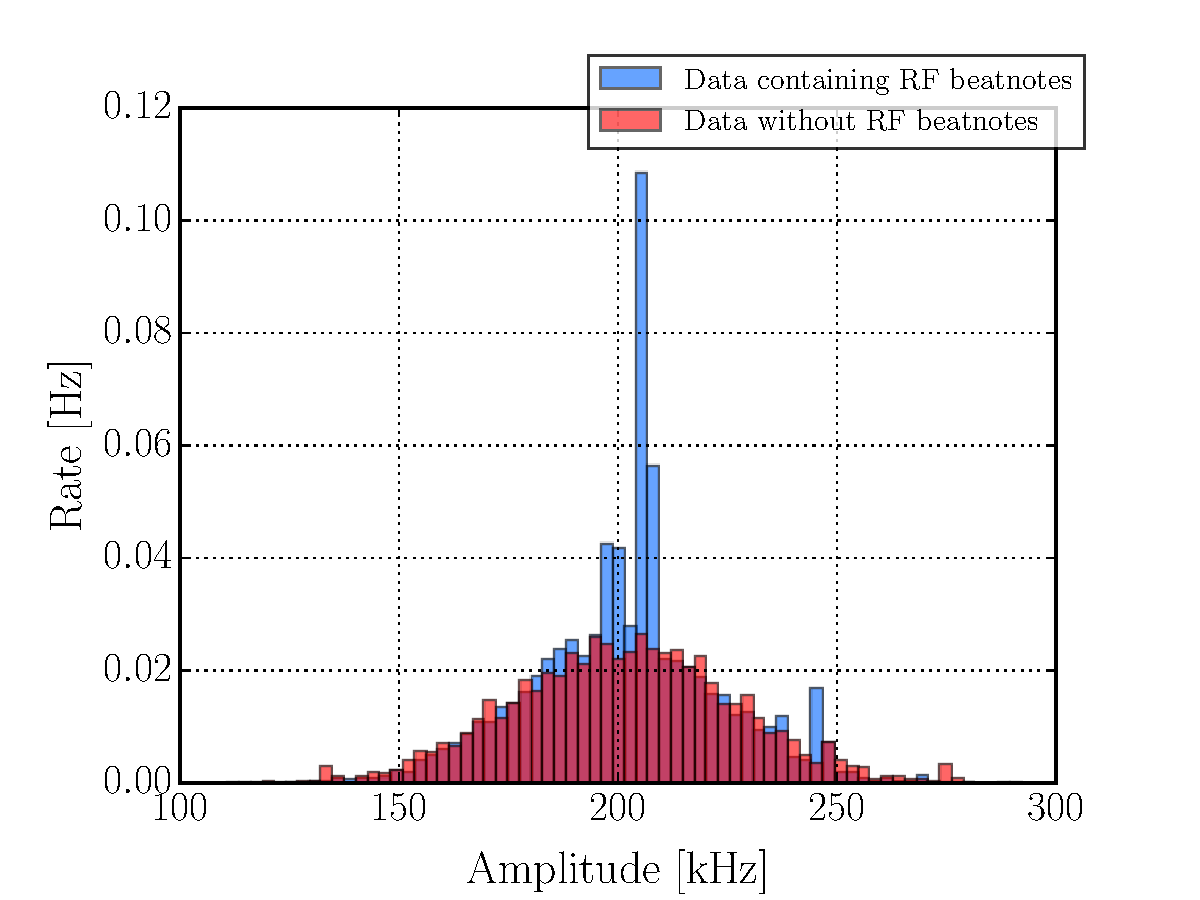
\includegraphics[width=\textwidth]{figures/detchar/Rate_Histogram_Whistles_LLO}
\caption[DARM glitch histograms with and without RF whistles]{The red distribution %
         shows the rate of Omicron in triggers in $h(t)$ when RF whistles are not % 
         present. The blue distribution shows the rate of Omicron triggers in $h(t)$ % 
         when RF whistles are occurring. The x-axis is the value of a channel that %
         represents the length of the input mode cleaner. When there are no whistle %
         glitches, there is no channel value for which Omicron triggers are more %
         likely to occur. When there are whistle glitches in $h(t)$, specific %
         values of the input mode cleaner length seem more likely to be coincident %
         with Omicron triggers in $h(t)$.}
\label{fig:darm-whistle-hist}
\end{figure}

The VCO that acts as a proxy to the length of the input mode cleaner is 
nominally set to 80 MHz. As the length of the input mode cleaner drifts, the 
oscillator frequency can be tuned by $\pm$ 1 MHz to track the length, resulting 
in a signal with a frequency of 79 - 81 MHz. It was found that these whistle 
glitches occurred when the VCO frequency swept through 79.2 MHz, which is the 
same frequency as an oscillator used to drive an acousto-optic modulator. 
The variable oscillator that was tracking the length of the input mode cleaner 
was drifting past the static oscillator at 79.2 MHz and creating whistle glitches 
that were visible in $h(t)$.  
To reduce the number of whistle glitches in $h(t)$, the oscillator frequencies 
were moved away from one another so that the static oscillator was outside 
of the range of the tunable oscillator.

Figure \ref{fig:hveto-whistles} demonstrates how prevalent whistle glitches were 
before the oscillator frequencies were shifted to avoid them. Figure 
\ref{fig:hveto-whistles} is a time-frequency scatter plot of Omicron triggers in 
$h(t)$. The blue dots represent all Omicron triggers generated for $h(t)$ over 
this stretch of time. The red crosses indicate that a given Omicron trigger was found 
to be coincident with an Omicron trigger generated for an auxiliary channel that 
was a capable witness for whistle glitches. Approximately 90\% of the glitches in 
$h(t)$ are vetoed by the witness channel, indicating that whistles were the dominant 
source of transient noise in $h(t)$ in this time period. 


\begin{figure}[ht!]%
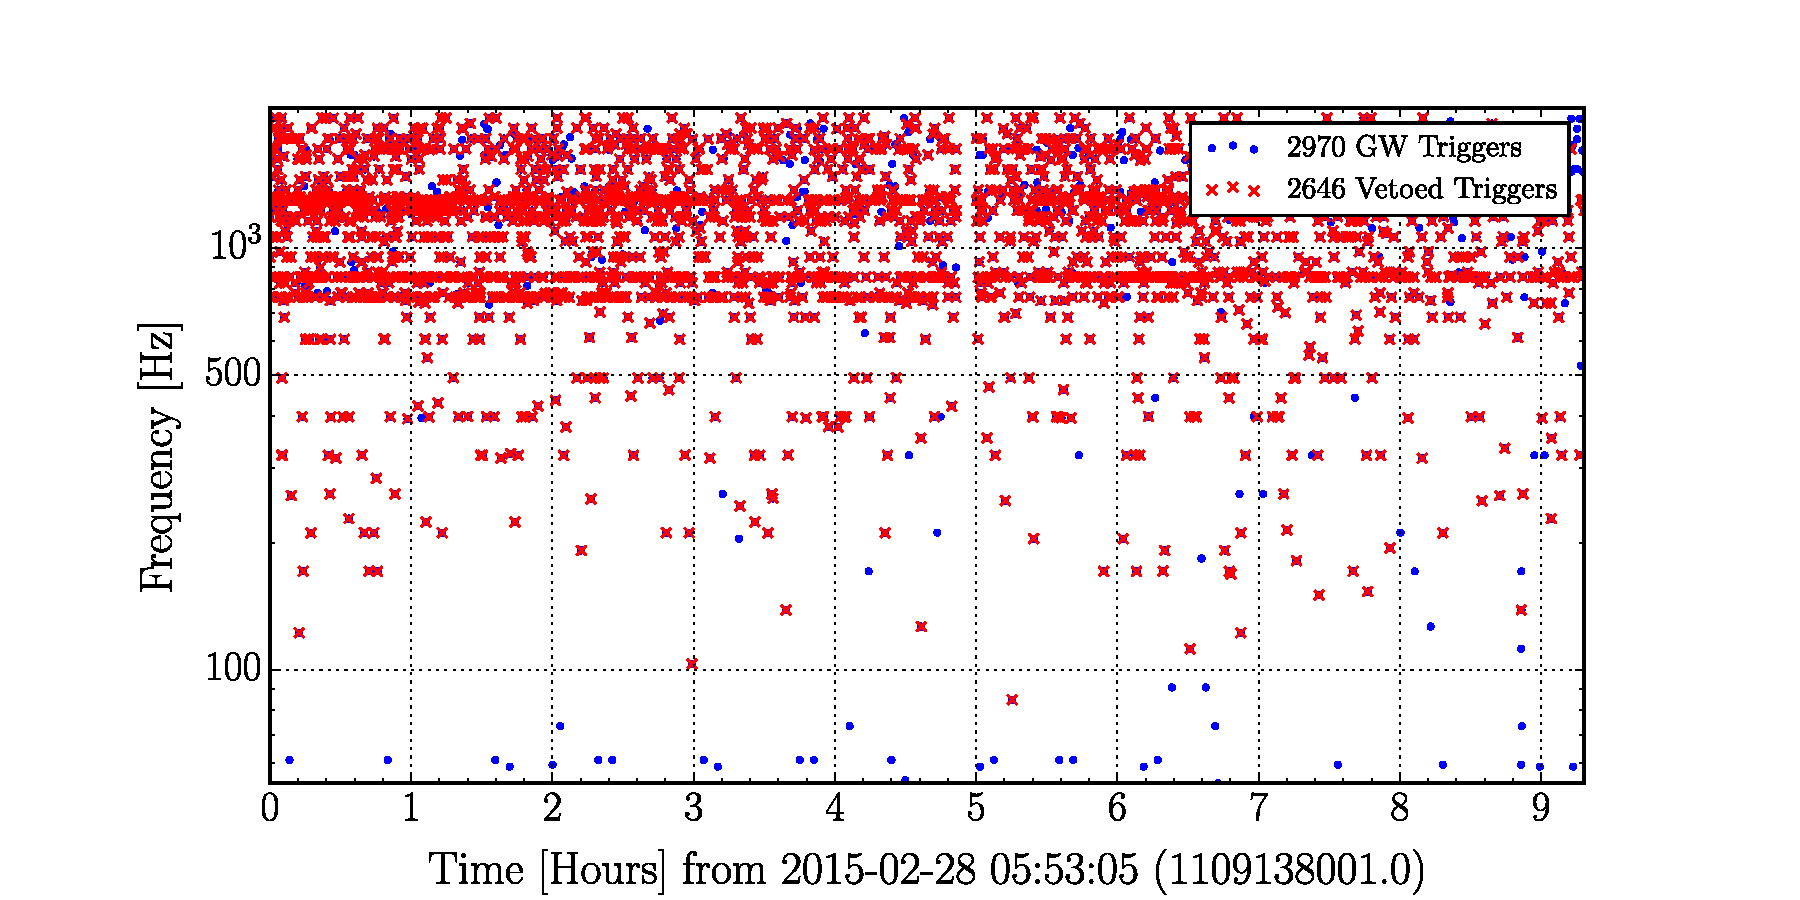
\includegraphics[width=\textwidth]{figures/detchar/Hveto_whistles_time_frequency}
\caption[Vetoed whistles from Hveto]{A time-frequency scatter plot of Omicron %
         triggers. The blue dots represent all triggers found for the $h(t)$ channel. %
         Red crosses indicate that a trigger was determined to be coincident with an %
         RF whistle and vetoed. This veto is responsible for removing 90\% of the %
         glitches in this time period. The majority of the high frequency glitches %
         were due to RF beatnote whistles}
\label{fig:hveto-whistles}
\end{figure}

The shape of the whistle 
glitches was also very problematic for CBC searches since the second half of a 
whistle is a sinusoid with a monotonically increasing frequency, not unlike the 
characteristic 'chirp' signal produced by a CBC event. Certain CBC waveforms 
matched the shape of the whistle glitches well enough to fool the $\chi^2$ signal 
consistency test and produced loud background triggers in early CBC searches. 
The whistle glitches 
were fixed before the first observing run, so they were not a limiting noise source 
to CBC searches during observation.

\subsection{Seismic CPS comb}

Oscillators in the capacitive position sensors had drifted apart and caused a 
beatnote and a comb. Audio analysis pointed towards amplitude modulation. 

Fixed by slaving all oscillators to a master.

\subsection{DC values of auxiliary channels}

No great correlation at the end of the day 

\subsection{Earthquakes during full lock}

Lots of scattering arches during an earthquake, drove up the noise and biased PSD.
Caused a sarlacc, removing this data was able to repair data on either side.

\subsection{L1 PMC glitches}


Characterization of noise and analysis after repair

\subsection{Data quality shifts}
Performed and mentored data quality shifts.

\section{Validation of Gravitational Wave Signals}\label{sec:GW150914-validation}

The Detector Characterization group was responsible for characterizing the 
noise in the interferometers in order to validate the gravitational 
wave signals GW150914 and GW151226. The first part of this analysis, which studied the 
stationarity of the background noise, is discussed in Section ?? . As a further 
check, the transient noise in the interferometer was also studied so that a 
confident detection claim could be made regarding GW150914. 

In the engineering runs leading up to the first observing run, a great deal of 
work was done to understand as much as possible about the noise coupling mechanisms 
from auxiliary channels into $h(t)$. Among the most important of these was a set 
of signal injections to test the sensitivity of the physical and environmental 
monitoring (PEM) subsystem. The PEM subsystem is comprised of a series of sensors 
that measure the ambient environmental noise at the interferometers. This 
subsystem is comprised of seismometers, accelerometers, magnetometers, radio 
antennae, microphones, temperature sensors, and voltage monitors for the power 
lines supplying the building. While the aLIGO detectors are extremely sensitive 
to external perturbations, they were built to be shielded against as many 
environmental disturbances as possible. In contrast, the PEM subsystem is comprised 
of extremely sensitive sensors that are more sensitive to environmental disturbances 
than the interferometer. By injecting signals into the interferometer enclosure, 
such as magnetic fields or acoustic vibrations, the relative sensitivity of the 
interferometer and the PEM sensors to environmental disturbances was established.

For both GW150914 and GW151226, the PEM subsystem reported that any environmental 
disturbances were at least 1 order of magnitude too weak to produce such an event. 
This includes electromagnetic transients, such as lightning strikes, that have the 
potential to generate coincident electromagnetic transients at L1 and H1. 

In addition to the checks performed in the PEM subsystem, a series of standard 
checks were done to ensure nominal performance in the interferometers. These 
checks are organized in a detection checklist, which gathers all of the 
relevant questions about interferometer performance that may influence 
gravitational wave detection. This list includes checks 
for the DAC calibration glitches mentioned in Section ??, the ADC and DAC 
digital saturation glitches mentioned in Section ??, coincidence with 
generic transients 
as reported by Omicron, time-frequency scans of all auxiliary channels to be 
investigated by DetChar subsystem leads, injections and test signals, and 
GPS or digital system timing errors. Each category was investigated and 
followed up on by the DetChar group and none of them gave significant 
reason to doubt the validity of GW150914 or GW151226.  
For both GW150914 and GW151226 there were small sets of auxiliary channels 
that showed excess power coincident with the 
gravitational wave signals, which is expected given the breadth of the auxiliary 
channel network, but after further investigation none of them had the 
necessary amplitude and frequency to generate an event similar to a CBC 
signal. 
